\chapter{\MakeUppercase{Methodology and Testing}}

\section{Methodology}

\begin{figure}[H]
	\centering
	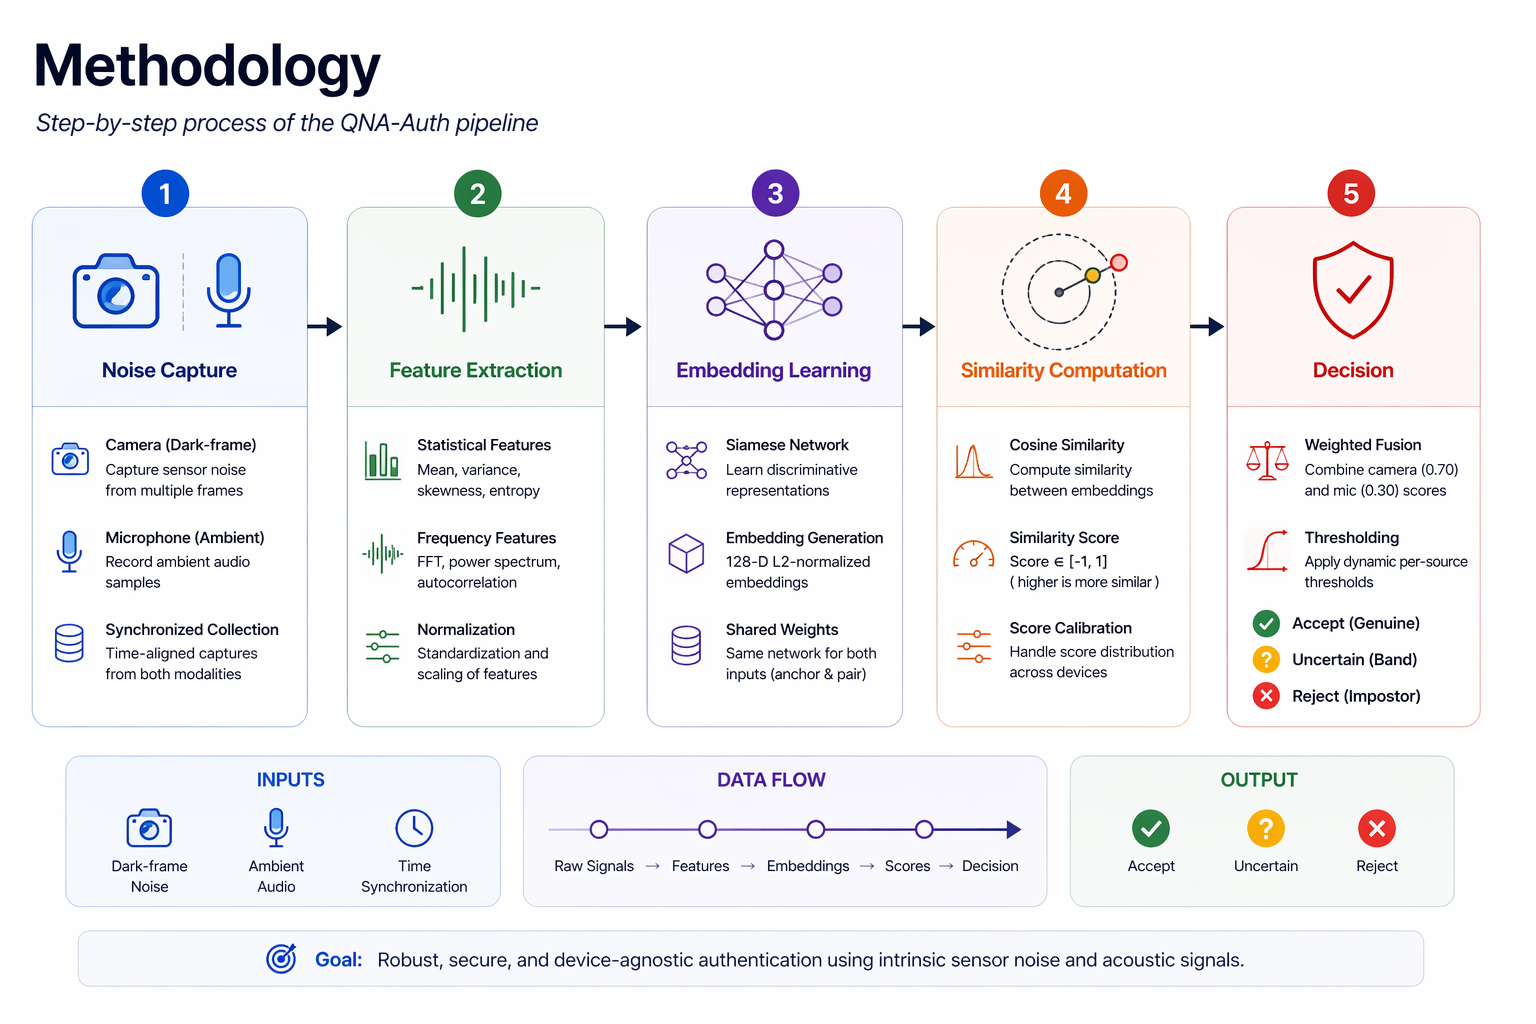
\includegraphics[width=0.95\linewidth]{images/methodology.png}
	\caption{Methodology of QNA-Auth}
	\label{fig:system_design}
\end{figure}

The five phases that define the QNA-Auth method are data acquisition, feature extraction, generation of embeddings, decision scoring, and verification at the level of individual systems. Explaining how the method achieves each of these phases (i.e., what the code does) also has to be justified as to why each of these phases fits together in both order and dependency.

\subsection{Noise Acquisition}
Camera and microphone are presently active sources for runtime. The backend captures samples directly from local hardware during the enrollment process, or they can accept sample array input from clients via the API. The direct collection method is best for live demonstrations, and client-provided payloads are used for testing and reproducibility, or provide alternative demonstrations. Authentication will work the same way in using both methods.

\subsection{Feature Extraction}
Reshaping each raw sample into a one-dimensional numeric array also includes scanning through those arrays for invalid entries. After this scanning occurs, each sample adds otherwise expensive transformation analysis views. Features are extracted from both the raw domain as well as the normalized domain of the sample data being analyzed. The combined hybrid design is preferred to a design that only includes normalized features since the adjectives associated with raw domain amplitude measurements still provide useful information regarding how the sample was measured.

\subsection{Embedding and Similarity}
A Siamese-like architecture is used to learn embeddings from the feature vectors; it consists of a multi-layer perceptron with degrees of freedom (Dof) at all hidden layers and a normalized output embedding of 128 dimensions at the last layer. Cosine similarity is the method used for measuring similarity. The runtime interface only uses the last layer of the model to get an embedding and the cosine similarity to compare embeddings (the system supports both triplet and contrastive configurations).

\subsection{Template Bank Construction}
The enrollment sample is stored in different ways rather than a single vector representation. The implementation consists of:
\begin{itemize}
	\item Source embeddings
	\item Source template banks
	\item Combined embeddings
	\item Combined template banks
\end{itemize}
Using a bank approach will provide enhanced robustness; i.e., each runtime sample could refer to multiple stored enrollment summaries, rather than using one "fragile" aggregated enrollment summary.

\subsection{Confidence Bands and Drift Updates}
The project creates a more flexible acceptance/rejection policy through the use of strong acceptance, uncertainty and rejects bands. By using this approach there is a better matching of weak sensor verification data than rigidly accepting or rejecting.
Additionally, this allows the system to request additional data samples or an alternative method to authenticate if there is not an adequate level of certainty for the evidence collected such that it can be considered accurate.

Template drift is handled through an ema update strategy gated by strong accepts. If $e_{old}$ is the stored embedding and $e_{auth}$ is a fresh strong-match embedding, the updated template is:
\begin{equation}
e_{new} = \frac{(1-\alpha)e_{old} + \alpha e_{auth}}{\|(1-\alpha)e_{old} + \alpha e_{auth}\|_2}
\end{equation}

Finally, the coding requirements for a minimum number of strong matches prior to performing an update helps to reduce the potential for gradual poisoning of the sensor data.

\section{Algorithms}
\begin{algorithm}[H]
	\caption{Enrollment algorithm}
	\label{alg:enrollment}
	\begin{algorithmic}
		\Require device name, sources, sample count
		\Ensure device template bundle persisted
		\State collect or receive noise samples by source
		\State extract canonical feature vectors for each sample
		\State generate source embeddings
		\State build source template bank from chunked samples
		\State combine source embeddings using configured weights
		\State compute metadata and source profiles
		\State save template bundle and metadata
	\end{algorithmic}
\end{algorithm}

\begin{algorithm}[H]
	\caption{Authentication algorithm}
	\label{alg:authentication}
	\begin{algorithmic}
		\Require claimed device, fresh samples
		\Ensure decision and diagnostics
		\State load stored record and metadata
		\State validate source set
		\State compute runtime source \ac{rms} profile
		\If{profile mismatch}
			\State reject
		\EndIf
		\State generate runtime embeddings
		\State score against stored template banks
		\State compute weighted similarity
		\State compute best impostor similarity
		\If{strong band and margin satisfied}
			\State accept
		\ElsIf{uncertain band}
			\State return uncertain
		\Else
			\State reject
		\EndIf
	\end{algorithmic}
\end{algorithm}

\section{Testing Strategy}
There are specific tests that are conducted to evaluate the model, selection rates of all users, determine if the features
have any form of drift, confirm feature importances, and perform authentication guards and margin checks. 

Testing in QNA-Auth can be grouped into four categories:
\begin{itemize}
	\item Preprocessing and feature consistency tests
	\item Model and evaluation tests
	\item Authentication-rule and guard tests
	\item Operational diagnostics and preflight scripts
\end{itemize}

